\documentclass[t,12pt]{beamer}
 %
 % Packages pour le français
 \usepackage[T1]{fontenc} 
 \usepackage[french]{babel}
 %
 % pour un pdf lisible à l'écran
 % il y a d'autres choix possibles 
 \usepackage{pslatex}
 %
\usepackage{caption}
\usepackage{subcaption}
 % pour le style et couleurs
 \usetheme{Boadilla}
 %
 
 %Path relative to the main .tex file 
\graphicspath{ {./images/} }

%Information to be included in the title page:
\title{Développement mobile}
\author{JAFFUER Pierre - LE LIDEC Tristan}
\date{Décembre 2021}

\begin{document}

\frame{\titlepage}


\begin{frame}{Introduction}
    Contexte : 
    \begin{itemize}
        \item UE développement mobile
        \item Application Android
        \item Java
    \end{itemize}
    
    Notions utilisées :
    \begin{itemize}
        \item Capteurs (accéléromètre)
        \item Gestes courants  (double tap et balayage vers le haut)
        \item Appareil photo
    \end{itemize}
\end{frame}

\section*{Sommaire}
\begin{frame}{Sommaire}
\tableofcontents
\end{frame}



\section{Idées}
\begin{frame}{Première idée}
    Un jeu de bataille navale :
    \begin{itemize}
        \item en 3D
        \item utilisation de AR core
        \item réalité virtuelle
    \end{itemize}
\end{frame}

\begin{frame}{Première idée}
    Les + :
    \begin{itemize}
        \item utilisation de beaucoup de capteurs
        \item gestuelle très utilisée
    \end{itemize}
    Les - :
    \begin{itemize}
        \item demande beaucoup de travail
        \item du temps
    \end{itemize}
\end{frame}

\begin{frame}{Idée réalisée}
    \begin{figure}
        \centering
        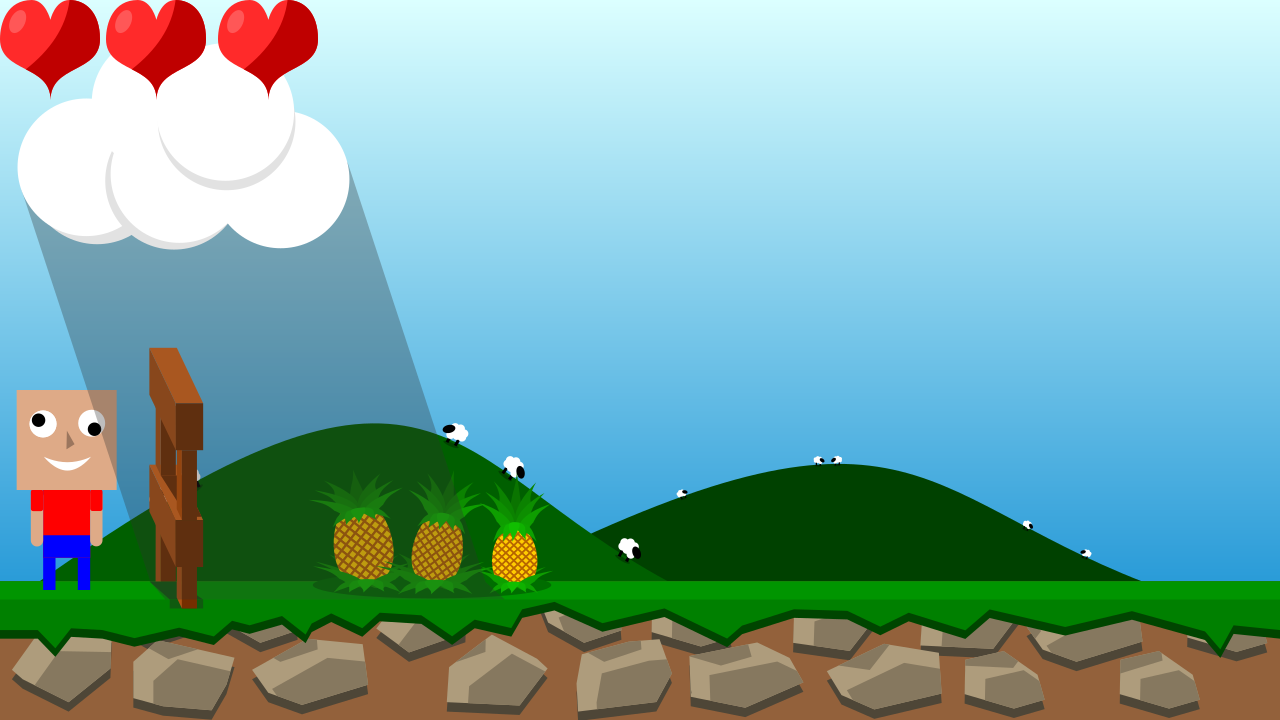
\includegraphics[width=1\linewidth]{images/game.png}
        \caption{Jumpy}
        \label{fig:jeu}
    \end{figure}
    
    Réalisation :
    \begin{itemize}
        \item graphismes : Inkscape
        \item audio : Audacity, BoscaCeoil, sfxr
        \item android vanilla
    \end{itemize}
\end{frame}

\begin{frame}{Idée réalisée}

    \begin{itemize}
        \item android vanilla
        \item MediaPlayer et SoundPool
    \end{itemize}

    Logiciels utilisés :
    \begin{itemize}
        \item graphismes : Inkscape
        \item audio : Audacity, BoscaCeoil, sfxr
    \end{itemize}
\end{frame}

\section{Le jeu}

\subsection{Le joueur}



\begin{frame}{Le joueur}
    Le joueur est divisé en 2 parties :
    \begin{itemize}
        \item La tête (Image personnalisable)
        \item Le corps
    \end{itemize}
    
\end{frame}

\subsubsection{La tête}
\begin{frame}{La tête}
    \begin{figure}
        \centering
        
\includegraphics{face}
        \caption{Tête par défaut du joueur}
        \label{fig:tete_joueur}
    \end{figure}
    \begin{itemize}
        \item Bitmap purement cosmétique
        \item Remplaçable par un selfie du joueur
    \end{itemize}
\end{frame}

\subsubsection{Le corps}
\begin{frame}{Le corps}
    \begin{figure}
        \centering
        
\includegraphics{corps_joueur}
        \caption{Corps du joueur}
        \label{fig:corps_du_joueur}
    \end{figure}
    \begin{itemize}
        \item collisions
        \item déplacements
    \end{itemize}
\end{frame}

\subsection{Gestion des collisions}
\begin{frame}{Gestion des collisions}
Pool d'objets
\begin{figure}[h]
    \centering
    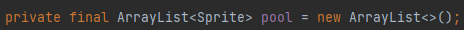
\includegraphics[scale=0.8]{poolObjets}
    \caption{Instanciation pool objets}
    \label{fig:instanciation pool objets}
\end{figure}
    
\end{frame}

\begin{frame}{Gestion des collisions}
    \begin{figure}[h]
        \centering
        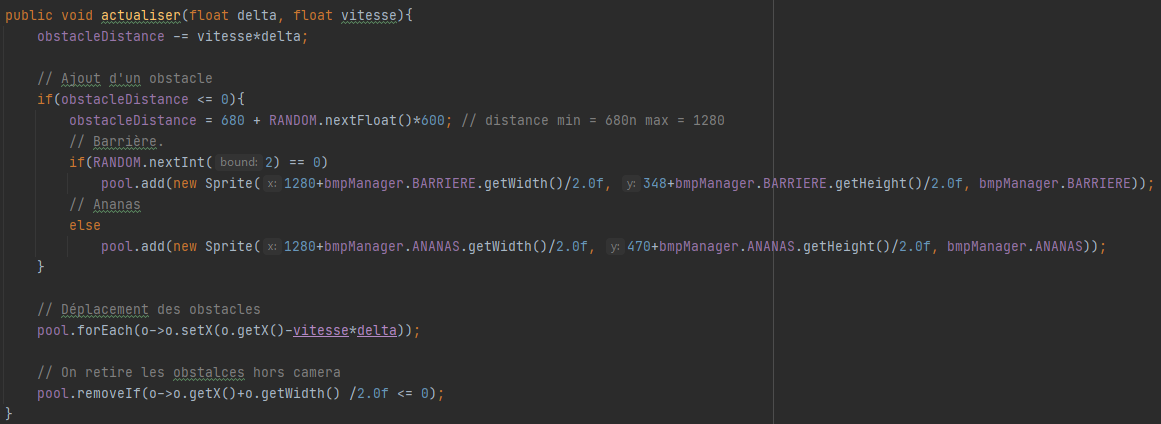
\includegraphics[scale=0.37]{actuObjets}
        \caption{Actualisation du pool d'objets}
        \label{fig:ajout des objets}
    \end{figure}
\end{frame}

\begin{frame}{Gestion des collisions}
    \begin{figure}[h]
        \centering
        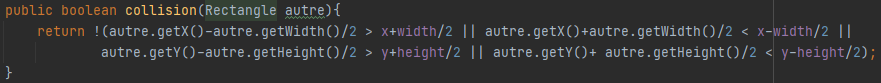
\includegraphics[scale=0.5]{fctColl}
        \caption{Détection de collision}
        \label{fig:my_label}
    \end{figure}
\end{frame}

\begin{frame}{Gestion des collisions}
    \begin{figure}[h]
        \centering
        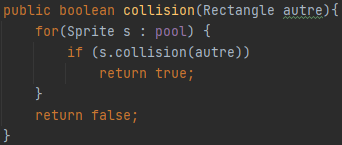
\includegraphics{collision}
        \caption{Collision entre des sprites}
        \label{fig:collision entre sprite}
    \end{figure}
\end{frame}

\section{Le dessin}
\begin{frame}{Le dessin}
    Utilisation d'un canvas pour tout le jeu
    
    \begin{itemize}
        \item surfaceView
        \item canvas GPU (Android 8)
        \item Thread d'actualisation
    \end{itemize}
    
    \begin{figure}
     \centering
     \begin{subfigure}[b]{0.2\textwidth}
         \centering
         
\includegraphics[width=\textwidth]{nuage}
         \caption{Nuage}
         \label{fig:Nuage}
     \end{subfigure}
     \hfill
     \begin{subfigure}[b]{0.2\textwidth}
         \centering
         
\includegraphics[width=\textwidth]{ciel}
         \caption{ciel}
         \label{fig:ciel}
     \end{subfigure}
     \hfill
     \begin{subfigure}[b]{0.2\textwidth}
         \centering
         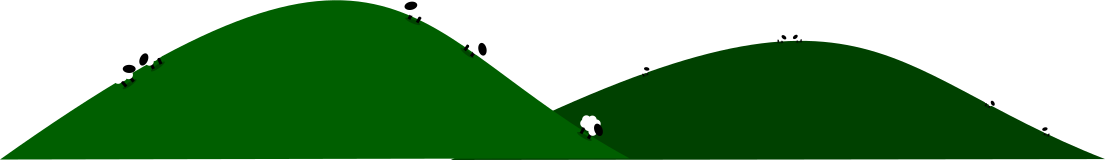
\includegraphics[width=\textwidth]{collines}
         \caption{collines}
         \label{fig:collines}
     \end{subfigure}
     \hfill
     \begin{subfigure}[b]{0.2\textwidth}
         \centering
         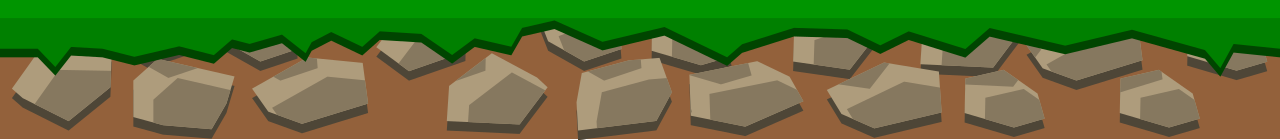
\includegraphics[width=\textwidth]{sol}
         \caption{sol}
         \label{fig:sol}
     \end{subfigure}
     \caption{Nos assets}
     \label{fig:three graphs}
    \end{figure}
\end{frame}

\subsection{Les obstacles}
\begin{frame}{Les obstacles}
    \begin{figure}
     \centering
     \begin{subfigure}[b]{0.3\textwidth}
         \centering
         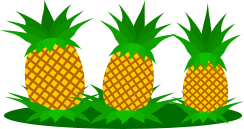
\includegraphics[scale=0.5]{ananas}
         \caption{Ananas}
         \label{fig:Ananas}
     \end{subfigure}
     \hfill
     \begin{subfigure}[b]{0.1\textwidth}
         \centering
         
\includegraphics[scale=0.5]{barriere}
         \caption{Barriere}
         \label{fig:Barriere}
     \end{subfigure}
     \caption{Obstacles}
     \label{fig:obstacles}
    \end{figure}
\end{frame}

\section{Gestes et capteurs}
\subsection{La gestuelle}
\begin{frame}{La gestuelle}
    \begin{itemize}
        \item double tap
        \item glissement vers le haut
    \end{itemize}
\end{frame}

\subsubsection{Double tap}
\begin{frame}{Double tap}

\begin{figure}
    \centering
    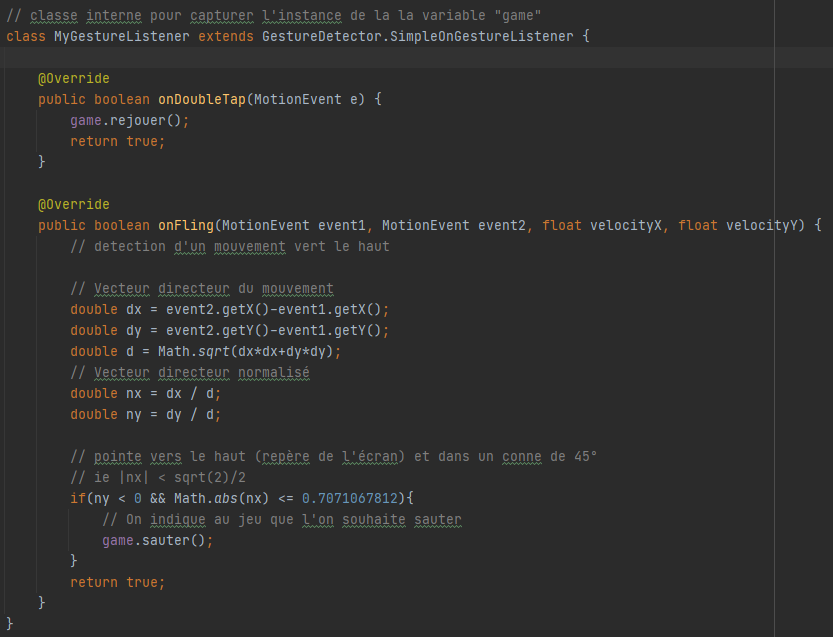
\includegraphics[width=0.75\linewidth]{images/gesture.png}
    \caption{Classe fille SimpleOnGestureListener}
\end{figure}

    
\end{frame}

\subsubsection{Glissement ver le haut}
\begin{frame}{Glissement vers le haut}

\begin{figure}
    \centering
    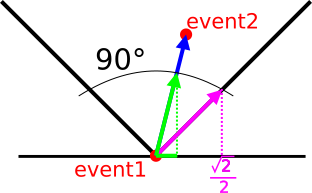
\includegraphics{images/swipe_up.png}
    \caption{Détection d'un balayage vers le haut}
\end{figure}
\end{frame}

\subsection{Les capteurs}
\begin{frame}{Les capteurs}
    \begin{itemize}
        \item Accéléromètre
        \item appareil photo
    \end{itemize}
\end{frame}

\subsubsection{Accéléromètre}
\begin{frame}{Accéléromètre}

\begin{figure}
    \centering
    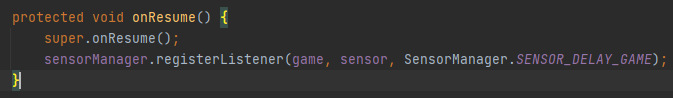
\includegraphics[width=1\linewidth]{images/accéléro.png}
    \caption{Accéléromètre}
    \label{fig:accelero}
\end{figure}
    
\end{frame}

\subsubsection{Appareil photo}
\begin{frame}{Appareil photo}
    Vérification des permissions impérative.
    \begin{figure}
     \centering
     \centering
     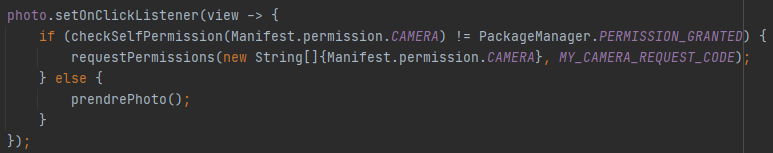
\includegraphics[scale=0.5]{clickPhoto}
     \caption{Bouton pour prendre une photo}
     \label{fig:Bouton photo}
    \end{figure}
\end{frame}

\begin{frame}{Appareil photo}
    Invocation à une application de caméra déjà installée.
    \begin{figure}
        \centering
        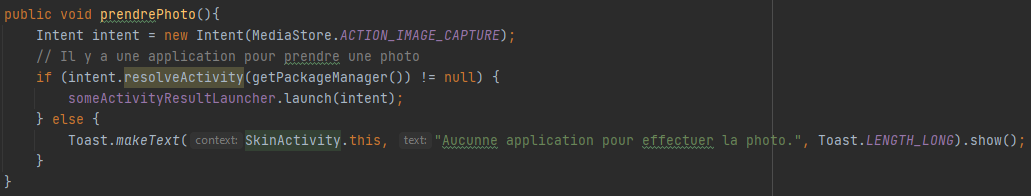
\includegraphics[scale=0.4]{takePhoto}
        \caption{Caption}
        \label{fig:my_label}
    \end{figure}
\end{frame}

\section{Interface}
\begin{frame}{Interface}
Traduction anglaise et française de l'UI.
\begin{figure}
    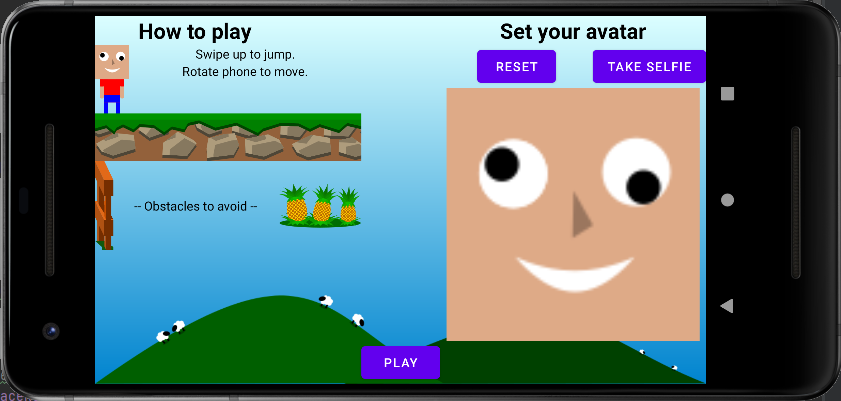
\includegraphics[width=0.5\linewidth]{images/selfie_horizontal.png}
    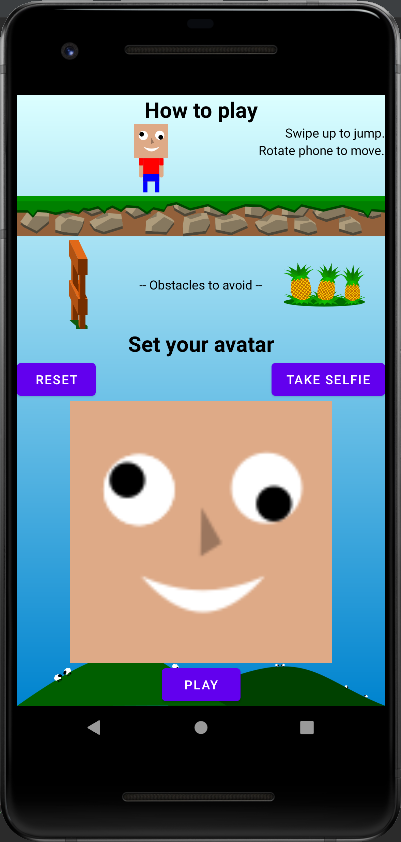
\includegraphics[height=0.5\linewidth]{images/selfie_vertical.png}
    \caption{Adaptation à l'orientation}
\end{figure}
\end{frame}

\begin{frame}{Conclusion}
\begin{itemize}
    \item Utilisation de capteurs
    \item simple mais fonctionnel
    \item Gestion des compromis
\end{itemize}
\end{frame}

\begin{frame}{démonstration}
\centering
    \Huge démonstration
\end{frame}

\end{document}